\chapter{Results and Analysis}
Every number in this chapter is taken from the evaluation files committed in the \texttt{results/} folder of the repository: the bias model evaluation written by the training script, the simulator evaluation, the causal results, and the paper evaluation written by \texttt{evaluate\_for\_paper.py}. The charts were plotted directly from these files. The experiments use fixed seeds and cached market data, so they can be reproduced. The behavioral labels are synthetic and the market history is real; no experiment with real investors has been carried out.

\section{Experimental Setup}
The 20,000 cases of dataset v4.1 were split into 16,000 development and 4,000 test cases, stratified by label and market regime, and the test set was used once. Five-fold cross-validation with early stopping on the development set gave best iterations of 423, 330, 329, 381 and 364, and the final model uses 402 trees (1.1 times the mean). Because stress regimes are over-sampled, every metric is re-weighted to the real frequency of each regime (normal 39.4\%, bull 29.0\%, correction 19.9\%, crash 6.6\%, euphoria 5.2\%), and these are the figures quoted throughout.

\begin{table}[H]
\centering
\small
\begin{tabular}{|l|l||l|l|}
\hline
\textbf{Hyperparameter} & \textbf{Value} & \textbf{Hyperparameter} & \textbf{Value} \\
\hline
Objective & multi:softprob & Row subsample & 0.85 \\
\hline
Number of trees & 402 & Column subsample & 0.85 \\
\hline
Maximum depth & 5 & Minimum child weight & 3 \\
\hline
Learning rate & 0.03 & L2 regularization ($\lambda$) & 2.0 \\
\hline
Tree method & hist & Split seed / model seed & 7 / 42 \\
\hline
\end{tabular}
\caption{Hyperparameters of bias model v4.1}
\label{tab:hyper}
\end{table}

The evaluation metrics are accuracy, per-class precision, recall and F1, macro-F1 (the mean of the per-class F1 scores, which gives each class equal weight since loss aversion is only 10\% of cases), log-loss and the expected calibration error defined in Chapter 5. With weighted counts of true positives $TP_k$, false positives $FP_k$ and false negatives $FN_k$:
\begin{equation}
\text{Precision}_k = \frac{TP_k}{TP_k + FP_k}, \qquad \text{Recall}_k = \frac{TP_k}{TP_k + FN_k},
\end{equation}
\begin{equation}
F1_k = \frac{2\,\text{Precision}_k\,\text{Recall}_k}{\text{Precision}_k + \text{Recall}_k}.
\end{equation}

\section{Behavioral Classification Results}
\begin{table}[H]
\centering
\small
\begin{tabular}{|l|c|c|}
\hline
\textbf{Metric} & \textbf{As sampled} & \textbf{Real frequency} \\
\hline
Accuracy (test) & 86.0\% & \textbf{87.9\%} \\
\hline
Macro-F1 (test) & 0.834 & \textbf{0.840} \\
\hline
Expected calibration error (test) & -- & \textbf{0.014} \\
\hline
Log-loss (test) & -- & 0.246 \\
\hline
Cross-validation accuracy & 84.9\% & 86.3\% \\
\hline
Patterns the definitions rule out & -- & 0\% \\
\hline
\end{tabular}
\caption{Overall test performance of the bias model}
\label{tab:overall}
\end{table}

\begin{figure}[H]
\centering
\begin{minipage}[t]{0.49\textwidth}
\centering
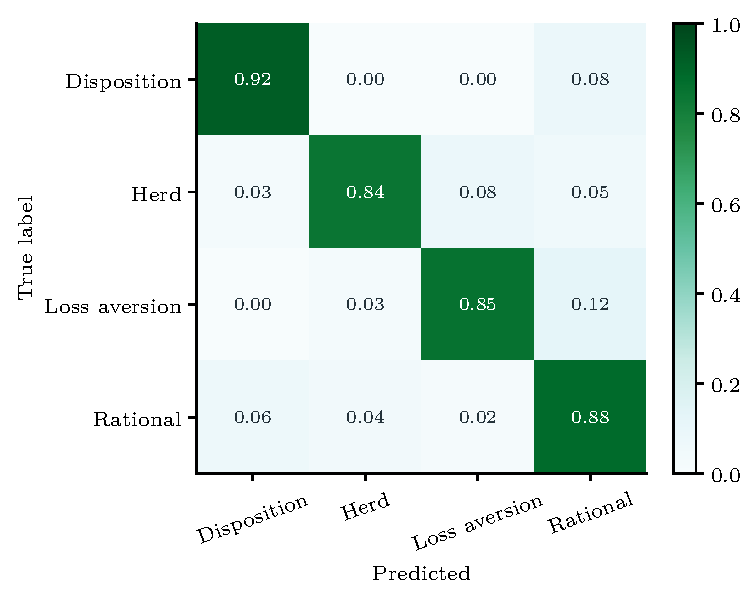
\includegraphics[width=\textwidth]{figures/charts/confusion.pdf}
\caption{Confusion matrix (rows normalized, real frequency)}
\label{fig:confusion}
\end{minipage}\hfill
\begin{minipage}[t]{0.47\textwidth}
\centering
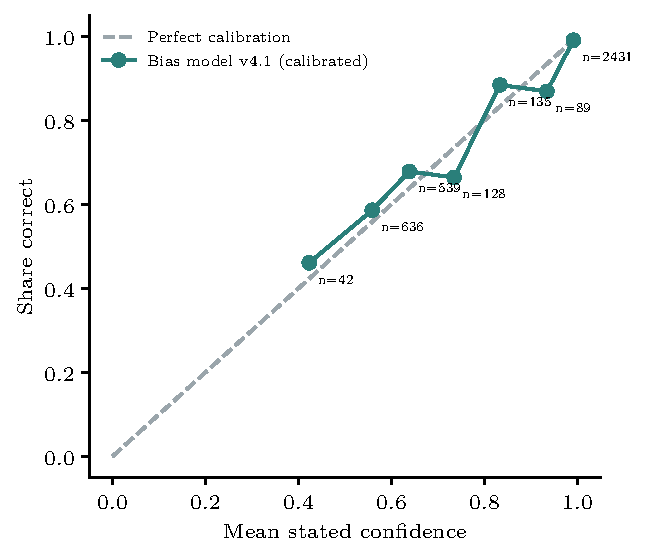
\includegraphics[width=\textwidth]{figures/charts/reliability.pdf}
\caption{Reliability diagram after calibration}
\label{fig:reliability}
\end{minipage}
\end{figure}

\begin{table}[H]
\centering
\small
\begin{tabular}{|l|c|c|c|}
\hline
\textbf{Pattern} & \textbf{Precision} & \textbf{Recall} & \textbf{F1} \\
\hline
Disposition effect & 0.844 & 0.918 & 0.879 \\
\hline
Herd behavior & 0.819 & 0.838 & 0.828 \\
\hline
Loss aversion & 0.667 & 0.849 & 0.747 \\
\hline
Rational & 0.939 & 0.875 & 0.906 \\
\hline
\end{tabular}
\caption{Per-class metrics (real frequency)}
\label{tab:perclass}
\end{table}

Table \ref{tab:overall} gives the overall result: 87.9\% accuracy, macro-F1 of 0.840 and an expected calibration error of 0.014 on the test set. The guard and the calibration step did not change any prediction on the test set. Table \ref{tab:perclass} and Figure \ref{fig:confusion} show that loss aversion is the weakest class. In a falling and fearful market, a loss-making sale is permitted under both loss aversion (panic) and herd behavior (selling into fear), and the data cannot always tell which motive won: 8.0\% of true herd cases are read as loss aversion, and 12.2\% of true loss aversion cases are read as rational. Rational decisions are recognized with the highest precision (0.939). This matters because wrongly calling a sensible decision biased is the more harmful error for a user.

\begin{table}[H]
\centering
\small
\begin{tabular}{|l|c|c|c|}
\hline
\textbf{Band shown to the user} & \textbf{Threshold} & \textbf{Share of analyses} & \textbf{Share correct} \\
\hline
High & $\geq$ 0.85 & 68.4\% & \textbf{98.7\%} \\
\hline
Medium & 0.65 to 0.85 & 7.1\% & 74.4\% \\
\hline
Low & $<$ 0.65 & 24.5\% & 61.7\% \\
\hline
\end{tabular}
\caption{Confidence bands and how often each is right}
\label{tab:bands}
\end{table}

The calibrated points in Figure \ref{fig:reliability} lie close to the diagonal. Most cases (66\% by weight) fall in the 0.95 to 1.00 bin, where the model is right 99.1\% of the time. The bands in Table \ref{tab:bands} are what the investor sees: a High reading is right about 99 times in 100, while a Low reading usually means that two patterns are close to even. In 44.3\% of cases the definitions allow only one label (holding a winner in a calm market, for example, can only be rational), which flatters the overall figures. On the remaining 55.7\%, the cases that need judgement, accuracy is 78.3\%.

Accuracy is 89.5\% in normal markets, 87.8\% in bull markets and corrections, 90.3\% in euphoria and 77.6\% in crashes, where loss aversion and herd behavior overlap the most. By action it is 84.9\% for sales, 90.0\% for holds and 89.4\% for purchases. Trained only on decisions dated 2008 to 2019 and tested on 2020 to 2026, which includes the COVID crash, the model reaches 86.5\% accuracy and 0.826 macro-F1, close to the random-split result.

\subsection{Baselines and Other Learners}
\begin{table}[H]
\centering
\small
\begin{tabular}{|l|c|c|}
\hline
\textbf{Model (real-frequency test set)} & \textbf{Accuracy} & \textbf{Macro-F1} \\
\hline
Always ``rational'' & 57.5\% & -- \\
\hline
Previous model v3 (same test cases) & 53.4\% & 0.309 \\
\hline
Definitions only (call a bias whenever one can apply) & 85.2\% & 0.825 \\
\hline
v4.1 without the \texttt{allows} inputs & 87.6\% & 0.832 \\
\hline
\textbf{v4.1} & \textbf{87.9\%} & \textbf{0.840} \\
\hline
Ceiling: v4.1 also given the hidden tendencies & 90.0\% & 0.866 \\
\hline
\end{tabular}
\caption{Baselines, ablation and ceiling}
\label{tab:baselines}
\end{table}

Table \ref{tab:baselines} is important for reading the model honestly. Because the labels come from written definitions, a rules-only baseline already reaches 85.2\%, and the model's gain over it is 2.7 points. The value of the model is in two places. It disagrees with the rules in 9.6\% of cases and is then right 64\% of the time against 36\% for the rules, because it recognizes rebalancing, a near goal, cutting a loss and a stated need for cash. It also gives calibrated confidence, which the rules cannot. The ceiling of 90.0\% shows that about one case in ten cannot be resolved from what the app observes. The previous model v3 scored 53.4\% on the same cases because it did not see the action: across 600 test cases, changing only the action changed v4.1's answer in 83.7\% of them and v3's in none.

\begin{table}[H]
\centering
\small
\resizebox{\textwidth}{!}{\begin{tabular}{|l|c|c|c|c|}
\hline
\textbf{Model} & \textbf{Accuracy (5 seeds)} & \textbf{Accuracy, seed 7 [95\% CI]} & \textbf{XGBoost minus model} & \textbf{McNemar $p$} \\
\hline
Rules only & 84.4\% $\pm$ 0.6 & 85.2\% [83.9, 86.4] & +2.7 [+1.6, +3.8] & $2.4\times10^{-7}$ \\
\hline
Logistic regression & 84.9\% $\pm$ 0.4 & 85.5\% [84.2, 86.6] & +2.4 [+1.4, +3.4] & $1.0\times10^{-5}$ \\
\hline
Random forest & 87.0\% $\pm$ 0.5 & 87.6\% [86.5, 88.7] & +0.2 [$-$0.4, +0.9] & 0.096 \\
\hline
XGBoost & 87.2\% $\pm$ 0.6 & 87.8\% [86.7, 89.0] & -- & -- \\
\hline
\end{tabular}}
\caption{Learners compared on the same features and guard (5 split seeds; bootstrap CIs and McNemar tests on seed 7)}
\label{tab:learners}
\end{table}

\begin{figure}[H]
\centering
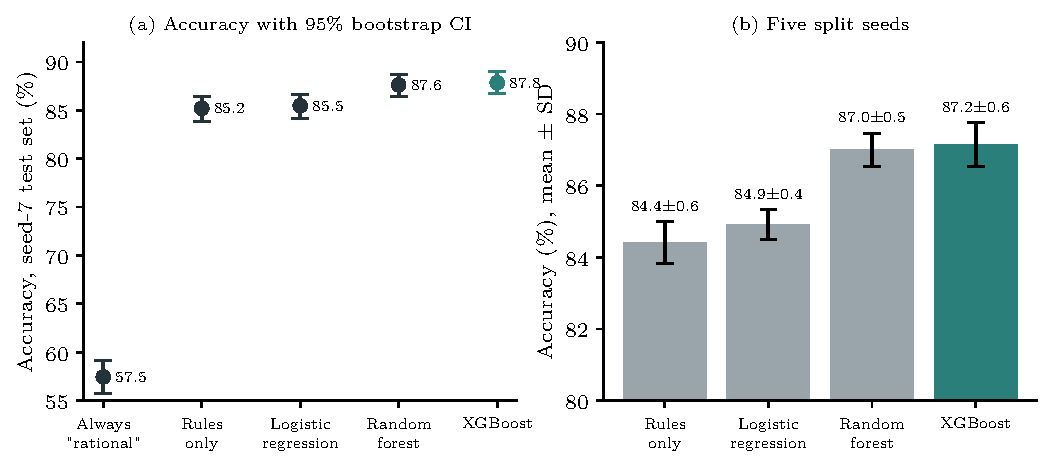
\includegraphics[width=0.95\textwidth]{figures/charts/baselines_ci.pdf}
\caption{(a) Accuracy with 95\% bootstrap confidence intervals; (b) mean and standard deviation over five split seeds}
\label{fig:learners}
\end{figure}

To check whether XGBoost is the right learner, logistic regression and a 500-tree random forest were trained on the same 22 features with the same guard and weighting, over five split seeds, with 2,000 bootstrap resamples and McNemar's test on the original split (Table \ref{tab:learners}, Figure \ref{fig:learners}). XGBoost is significantly better than the rules and logistic regression, which shows that the non-linear interactions matter. It is statistically tied with the random forest (a difference of 0.2 points with $p = 0.096$), so we do not claim that XGBoost is the better learner. It was kept because it has the lowest log-loss (0.267 against 0.282 for the forest), exact and fast TreeSHAP explanations and a portable model file.

Of the test cases, 167 are sales forced by money. Bias model v4.1 reads 71.9\% of them as rational: 90.6\% when the need is stated in the comment and 39.3\% when it is not, against 37.7\% for the earlier v4.0 model trained without money pressure. The gap between stated and unstated needs is exactly what the comment reader is designed to close. The training script also runs 13 scenario checks and 8 relational checks on a typical investor, and v4.1 passes all 21 (v3 passed 5 of the 13 scenarios). For example, selling a winner up 35\% in a calm market reads as the disposition effect with confidence 0.98, selling at a 20\% loss in a calm market reads as rational, and in a fearful market a stated cash need raises the rational reading from 0.09 to 0.49. Gold share alone barely moves the reading (largest change 0.05), as it should, since gold has no role in the label definitions.

\section{Simulator Results}
\subsection{Realism and Choice of Generator}
\begin{table}[H]
\centering
\small
\resizebox{\textwidth}{!}{\begin{tabular}{|l|c|c|c|c|c|}
\hline
\textbf{Generator} & \textbf{1-yr p10} & \textbf{1-yr median} & \textbf{1-yr p90} & \makecell{\textbf{ACF of squared}\\ \textbf{returns, lag 1/3/6}} & \textbf{KS distance} \\
\hline
Real NIFTY (217 windows) & $-$7.5\% & 11.3\% & 33.3\% & 0.136 / 0.051 / 0.093 & -- \\
\hline
Lognormal (GBM) & $-$16.2\% & 9.5\% & 42.1\% & $-$0.01 / $-$0.01 / $-$0.01 & 0.132 \\
\hline
Independent months & $-$15.9\% & 10.6\% & 41.2\% & $-$0.01 / $-$0.01 / $-$0.01 & 0.108 \\
\hline
Block 3 months & $-$14.3\% & 10.6\% & 37.8\% & 0.077 / $-$0.01 / $-$0.01 & 0.083 \\
\hline
Block 6 months & $-$13.7\% & 10.5\% & 35.9\% & 0.100 / 0.029 / $-$0.01 & 0.072 \\
\hline
\textbf{Block 12 months (used)} & \textbf{$-$8.1\%} & \textbf{10.3\%} & \textbf{33.1\%} & \textbf{0.101 / 0.035 / 0.025} & \textbf{0.027} \\
\hline
Block 24 months & $-$8.1\% & 10.3\% & 33.0\% & 0.105 / 0.023 / 0.033 & 0.030 \\
\hline
\end{tabular}}
\caption{Six market path generators against the real index (10,000 ten-year paths each, same historical mean)}
\label{tab:generators}
\end{table}

\begin{figure}[H]
\centering
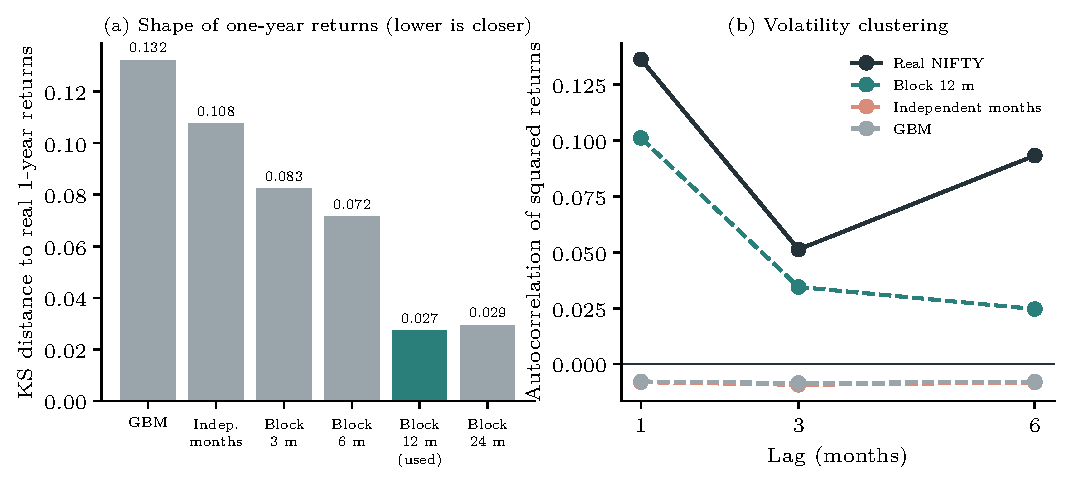
\includegraphics[width=0.95\textwidth]{figures/charts/generators.pdf}
\caption{(a) Kolmogorov-Smirnov distance to real one-year returns; (b) volatility clustering}
\label{fig:generators}
\end{figure}

Table \ref{tab:generators} and Figure \ref{fig:generators} justify the choice of generator. All six generators share the same average growth, so only the shape and the dependence differ. The 12-month block bootstrap is the only one that reproduces both the spread of real one-year returns and volatility clustering. Its KS distance (0.027) is a quarter of that of independent months (0.108) and a fifth of GBM's (0.132), while GBM and independent months have no clustering at all and make bad years about twice as bad as reality. Moving to 24-month blocks changes almost nothing. With the long-run growth assumptions used in the app, simulated one-year returns are $-$6.9\%, +11.6\% and +34.7\% at the 10th, 50th and 90th percentiles, against $-$7.5\%, +11.3\% and +33.3\% for the real index; the earlier v1 simulator had bad years of $-$15.8\%. The 19-year record holds only one independent decade, so ten-year comparisons (KS distance about 0.34 for every generator) are not used to rank generators.

\subsection{Effect of the Horizon and Stability of the Numbers}
\begin{table}[H]
\centering
\small
\begin{tabular}{|c|c|c|c|c|}
\hline
\textbf{Horizon} & \makecell{\textbf{Stock down 17\%:}\\ \textbf{holding wins}} & \textbf{Typical gap} & \makecell{\textbf{Fund up 30\%:}\\ \textbf{holding wins}} & \textbf{Typical gap} \\
\hline
1 year & 55\% & \rupee 3,592 & 66\% & \rupee 6,377 \\
\hline
3 years & 60\% & \rupee 13,950 & 70\% & \rupee 22,244 \\
\hline
5 years & 59\% & \rupee 21,124 & 70\% & \rupee 41,640 \\
\hline
10 years & 62\% & \rupee 59,925 & 75\% & \rupee 1.09 L \\
\hline
20 years & 64\% & \rupee 1.81 L & 80\% & \rupee 4.09 L \\
\hline
30 years & 61\% & \rupee 3.49 L & 81\% & \rupee 13.9 L \\
\hline
\end{tabular}
\caption{Effect of the horizon (\rupee 1 lakh position; investor earning \rupee 18 lakh a year with \rupee 11 lakh liquid)}
\label{tab:horizon}
\end{table}

\begin{figure}[H]
\centering
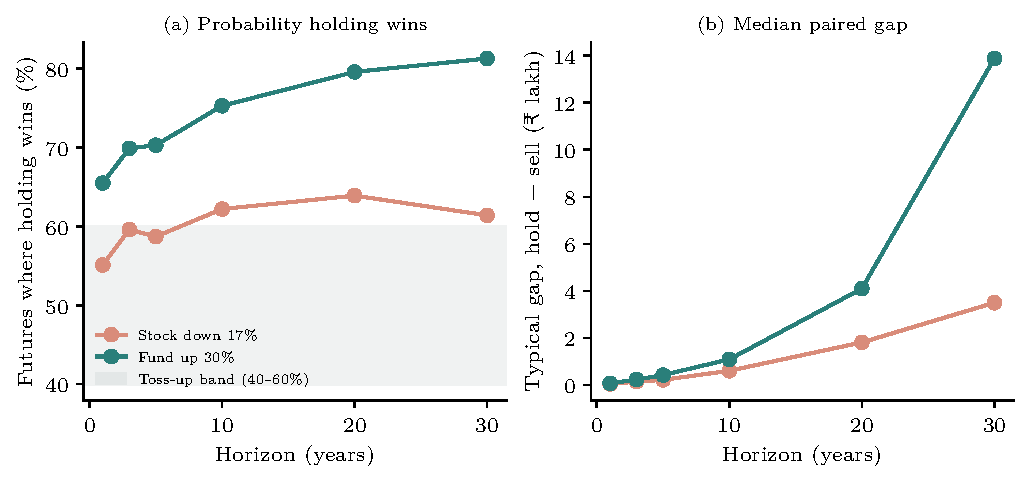
\includegraphics[width=0.95\textwidth]{figures/charts/horizon.pdf}
\caption{(a) Share of futures in which holding beats selling; (b) median paired gap, by horizon}
\label{fig:horizon}
\end{figure}

Table \ref{tab:horizon} and Figure \ref{fig:horizon} show the central practical result of the simulator. For a single stock down 17\%, the probability that holding beats selling stays between 55\% and 64\% at every horizon, mostly inside or near the band of 40 to 60\% that the recommendation rules treat as a toss-up. A diversified fund, with little company-specific risk, favors holding much more clearly and reaches 80\% at 20 years. The earlier simulator always used a 20-year horizon and therefore tilted every recommendation towards holding, even for someone who needs the money in three years.

\begin{figure}[H]
\centering
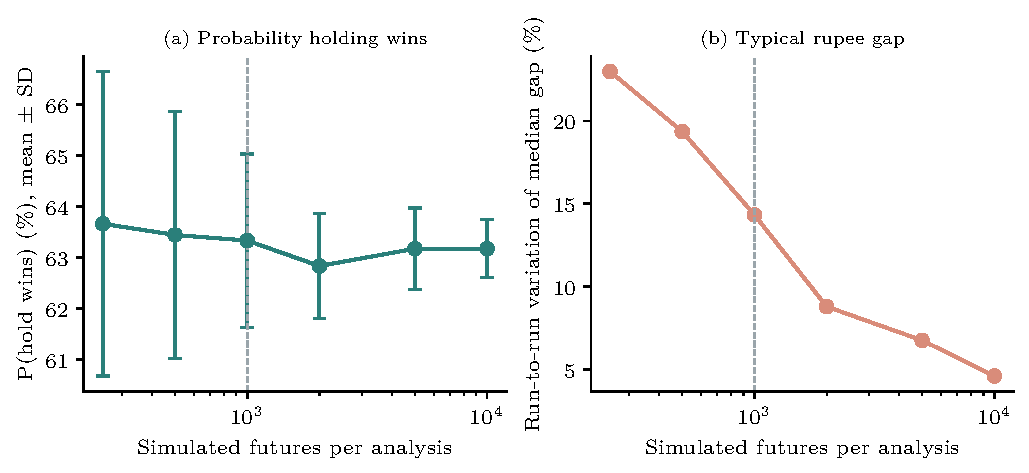
\includegraphics[width=0.95\textwidth]{figures/charts/convergence.pdf}
\caption{Monte Carlo convergence for the base case (20 repeats per size)}
\label{fig:convergence}
\end{figure}

Figure \ref{fig:convergence} shows how much of each number is simulation noise. At the app's 1,000 futures, the probability that holding wins (the input to the recommendation rules) varies by about $\pm$1.7 points between runs, close to the binomial standard error of $\pm$1.5 points. The median rupee gap is noisier and varies by about $\pm$14\%. This is why the verdict is driven by the probability and the rupee gap is presented as an approximate value.

\subsection{Results over 1,000 Investors and Sensitivity}
\begin{table}[H]
\centering
\small
\resizebox{\textwidth}{!}{\begin{tabular}{|l|c|c|c|}
\hline
\textbf{Group} & \textbf{Investors} & \textbf{Mean P(hold wins)} & \textbf{HOLD / toss-up / SELL} \\
\hline
All (long-run assumptions) & 1,000 & 0.635 & 58.1\% / 40.8\% / 1.1\% \\
\hline
Horizon 1 to 3 years & 52 & 0.571 & 29\% / 71\% / 0\% \\
\hline
Horizon 4 to 10 years & 100 & 0.598 & 43\% / 57\% / 0\% \\
\hline
Horizon 11 to 20 years & 275 & 0.624 & 57\% / 41\% / 2\% \\
\hline
Horizon 21 to 30 years & 573 & 0.652 & 64\% / 35\% / 1\% \\
\hline
Single stock & 596 & 0.562 & 31\% / 67\% / 2\% \\
\hline
Equity fund & 404 & 0.742 & 99\% / 1\% / 0\% \\
\hline
History replayed exactly & 1,000 & 0.380 & 5.6\% / 37.8\% / 56.6\% \\
\hline
\end{tabular}}
\caption{Paired simulation over 1,000 investors drawn from dataset v4.1}
\label{tab:population}
\end{table}

\begin{figure}[H]
\centering
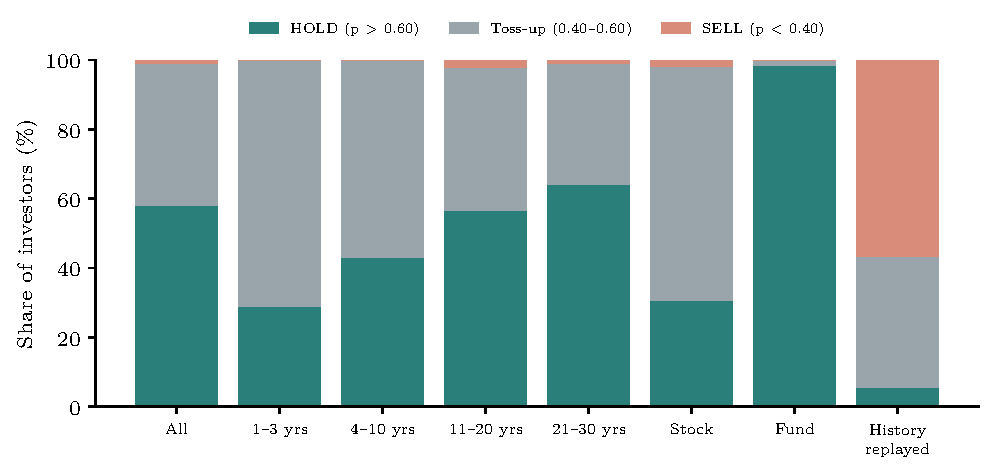
\includegraphics[width=0.9\textwidth]{figures/charts/population.pdf}
\caption{Share of investors in each verdict band}
\label{fig:population}
\end{figure}

Table \ref{tab:population} and Figure \ref{fig:population} move from single examples to a population. Under the long-run assumptions, holding is clearly favored for 58\% of investors, the comparison is a toss-up for 41\% and selling is favored for 1\%. Almost every equity fund (99\%) clearly favors holding, while only 31\% of single stocks do, because company-specific risk lowers the typical outcome. Whether the position is currently at a gain or a loss makes no difference (59\% and 57\% HOLD), which is exactly the point of the disposition effect literature: the purchase price should not matter for a forward-looking decision. The last row is the most important caution. If 2007 to 2026 is replayed exactly, gold compounds at about 15\% a year instead of 9\%, and 86\% of verdicts change.

\begin{figure}[H]
\centering
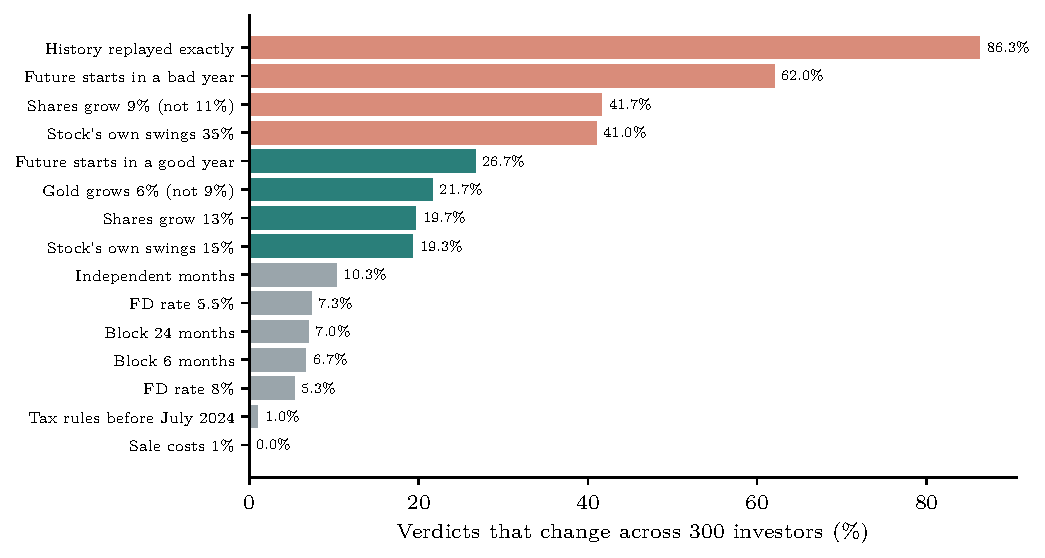
\includegraphics[width=0.85\textwidth]{figures/charts/sensitivity.pdf}
\caption{Share of verdicts that change across 300 investors when one assumption is changed}
\label{fig:sensitivity}
\end{figure}

Figure \ref{fig:sensitivity} ranks the assumptions by how many verdicts they change. The answer depends most on the growth assumptions for shares and gold (shares growing at 9\% instead of 11\% changes 41.7\% of verdicts), on how volatile the particular stock is (own volatility of 35\% instead of 21\% changes 41.0\%) and on the kind of year the future starts in (a bad first year changes 62.0\%). It barely depends on the block length, the July 2024 tax change (1.0\%) or sale costs (0\%, since the cost is charged on cashing out in both futures). This is why Folium measures each stock's risk at submission instead of assuming it, and why the growth assumptions are stated on every result page.

\begin{figure}[H]
\centering
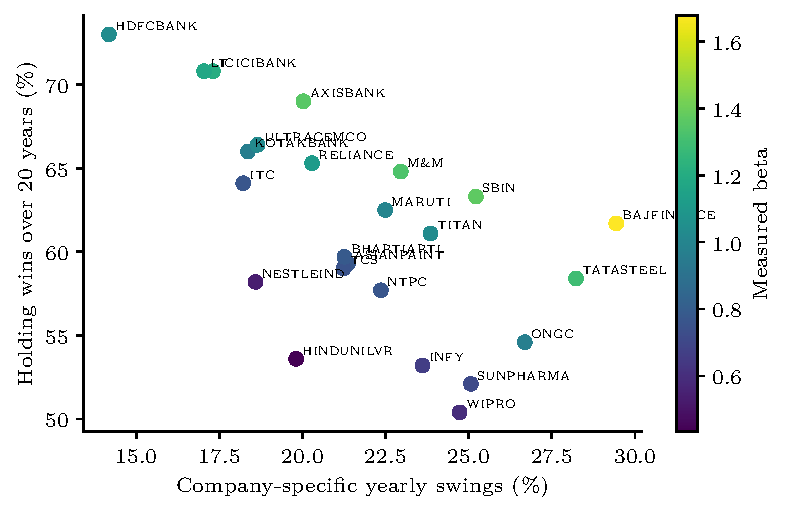
\includegraphics[width=0.75\textwidth]{figures/charts/stocks.pdf}
\caption{Company-specific volatility against the share of 20-year futures in which holding wins, for 24 NIFTY 50 stocks}
\label{fig:stocks}
\end{figure}

Figure \ref{fig:stocks} shows a clear negative relationship between a stock's own volatility and the advantage of holding it. HDFC Bank, with beta 1.03 and own volatility of 14\%, wins in 73\% of 20-year futures, while Wipro, with beta 0.60 and own volatility of 25\%, wins in 50\%. Two effects combine: own volatility drags down the median compound outcome, and a low beta lowers expected growth under the capital asset pricing relation. The second effect is a modeling choice, since steady low-beta stocks have often done better historically than the relation predicts.

\subsection{Comparison with Real History}
\begin{table}[H]
\centering
\small
\resizebox{\textwidth}{!}{\begin{tabular}{|c|c|c|c|c|c|}
\hline
\textbf{Window} & \makecell{\textbf{Real windows}\\ \textbf{(independent)}} & \makecell{\textbf{Hold won,}\\ \textbf{real}} & \makecell{\textbf{Hold won,}\\ \textbf{simulated}} & \makecell{\textbf{Real median}\\ \textbf{gap}} & \makecell{\textbf{Real inside simulated}\\ \textbf{10--90\% band}} \\
\hline
5 years & 169 (3) & 88.8\% & 61.0\% & \rupee 56,378 & 99.4\% \\
\hline
10 years & 109 (1) & 100\% & 60.7\% & \rupee 1,25,114 & 100\% \\
\hline
\end{tabular}}
\caption{Walk-forward replay of a fund up 30\% through every real window}
\label{tab:walk}
\end{table}

Table \ref{tab:walk} places what actually happened in each real 5-year and 10-year window inside the simulated distribution for the same case. Every real outcome but one falls inside the simulated 10th to 90th percentile band, and real outcomes sit in the upper middle of the band, since 2007 to 2026 was a good period for holding equity. With only one to three independent windows this is a consistency check and not a validation of forecasting ability. A related check concerns the paired gap itself: for the base-case investor over 14 years, the difference of the two medians and the median of the paired differences differ by up to 19\% at year 10 (\rupee 63,790 against \rupee 51,717). Folium reports the paired gap with its 10th to 90th percentile range ($-$\rupee 1,19,371 to \rupee 5,12,349 at year 10), because that range also shows that holding loses in a substantial share of futures even when it wins in the typical one.

\section{Cause and Effect Results}
\begin{table}[H]
\centering
\small
\resizebox{\textwidth}{!}{\begin{tabular}{|l|l|c|c|c|}
\hline
\textbf{Factor} & \textbf{Change} & \textbf{Sell} & \textbf{Hold} & \textbf{Buy more} \\
\hline
A cash shock & having one vs not & +31.8 (+31.3) & $-$23.6 ($-$23.3) & $-$8.2 ($-$8.0) \\
\hline
Emergency fund & having one vs not & $-$7.5 ($-$5.6) & +1.4 ($-$0.1) & +6.1 (+5.7) \\
\hline
Market fear & VIX +10 points & +6.4 (+3.9) & $-$4.7 ($-$2.9) & $-$1.7 ($-$1.0) \\
\hline
Weaker NIFTY month & 5 points worse & +5.6 (+5.8) & $-$3.9 ($-$3.7) & $-$1.7 ($-$2.1) \\
\hline
Bigger holding & +10 points of liquid & +4.8 (+4.7) & +2.7 (+2.8) & $-$7.5 ($-$7.5) \\
\hline
Longer horizon & +5 years & $-$2.4 ($-$2.3) & +1.4 (+1.4) & +1.0 (+1.0) \\
\hline
Gold (negative control) & +10 points & 0.0 ($-$0.2) & 0.0 (+0.4) & 0.0 ($-$0.2) \\
\hline
\end{tabular}}
\caption{Average effects in percentage points: true value, with the g-computation estimate in brackets}
\label{tab:effects}
\end{table}

\begin{figure}[H]
\centering
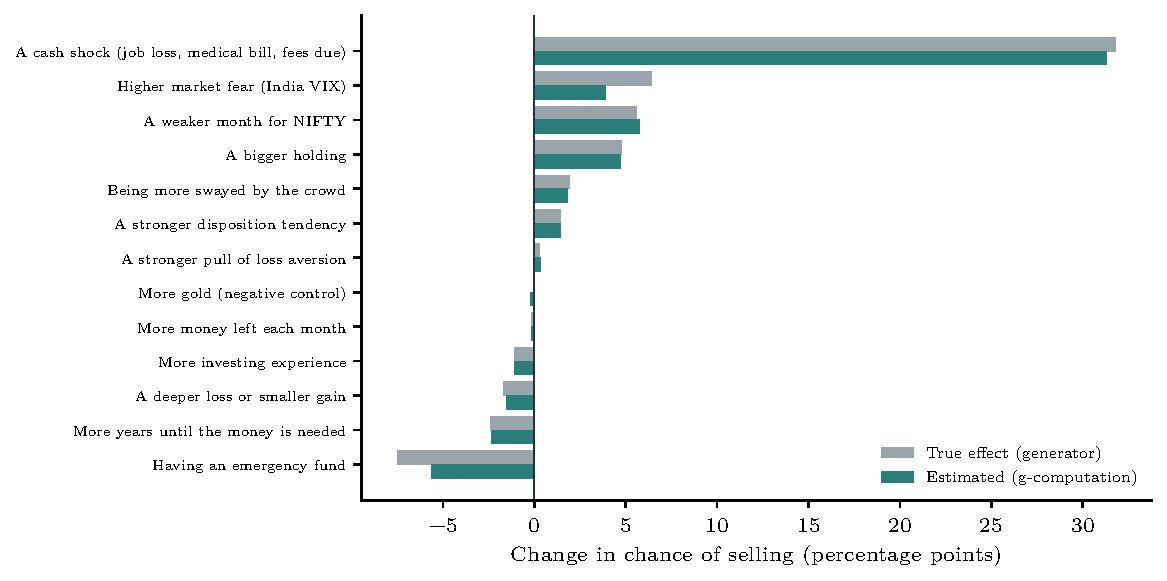
\includegraphics[width=0.92\textwidth]{figures/charts/causal.pdf}
\caption{Effect of each factor on the chance of selling: true effect against the g-computation estimate}
\label{fig:causal}
\end{figure}

Table \ref{tab:effects} and Figure \ref{fig:causal} show that money pressure dominates. A cash shock raises the chance of selling by about 32 points, and an emergency fund lowers it by 7.5 points, mostly by absorbing shocks. Market fear and a weak month push towards selling, and a bigger holding pushes towards selling (largely through rebalancing) and strongly away from adding. Loss aversion's population-wide effect is small (+0.3 points) because it acts only in specific situations; within them it is large.

Across all 45 effects, the g-computation estimates have a mean absolute error of 0.48 points and the correct direction in 97\% of cases. For effects on selling, g-computation's error is 0.45 points against 1.07 for the linear DoWhy model, which for example overstates the effect of investing experience about fivefold. The linear model is better at the effect of a tendency within its own situation (0.3 points against 1.4). DoWhy passed 12 of 13 refutation tests; the one failure is the gold negative control, whose true effect is zero, so a test against chance cannot confirm anything. When the most helpful habit is applied in each situation, the estimates always move in the right direction and, where they are off, they understate the benefit. For example, setting selling rules in advance lowers the share of winners sold in a calm market from 56\% to 39\% in truth, and the estimate gives 54\% to 40\%. One unexpected finding is that habits can work against each other: for someone holding a deep loser, all three habits together barely help (43\% to 42\%), while reframing the loss alone helps a lot (43\% to 36\%). For this reason the app offers the single most helpful habit and never a bundle.

\section{Explanation Quality}
Explanation quality was measured on the current pipeline for 166 sell and hold decisions drawn from the population study, explained in both English and Hindi (332 explanations), with AI wording switched off. Every explanation was complete (all six sections present), actionable and personalized, and none contained a jargon term. The English explanations have a mean Flesch reading ease of 76.4 (minimum 73.5, against a target of 60), which corresponds to fairly easy text, with 11.3 words per sentence. The Hindi explanations average 12.8 words per sentence against a target of 20; Flesch is not used for Hindi because its syllable model is undefined for Devanagari. These are measures of structure and readability; they do not show that the explanations change investor behavior, which would need a user study.

\section{Application Screenshots}
The screenshots in this section are to be captured from the running application with the demonstration accounts created by \texttt{scripts/seed\_demo.py}.

\newcommand{\screenshot}[2]{%
\begin{figure}[H]
\centering
\fbox{\parbox[c][5.2cm][c]{0.8\textwidth}{\centering\textit{Screenshot to be inserted}\\[4pt]#1}}
\caption{#2}
\end{figure}}
\screenshot{Result page}{Result page with the recommendation, both futures and the pattern found}
\screenshot{Live progress}{Live five-step progress during an analysis}
\screenshot{Hindi explanation}{Six-part explanation in Hindi}
\screenshot{Portfolio page}{Portfolio page with net worth, allocation and holdings}
\screenshot{Verify this record}{Verification of an audit record}
\screenshot{Google sign-in and Welcome page}{Google sign-in return and the Welcome profile step}

\section{Discussion}
On the development task, each analytical component does what it was designed to do. The classifier is accurate, calibrated and consistent with the label definitions, significantly better than the rules and a linear model and on par with a random forest. It changes its reading when the action changes, recognizes forced sales when the need is stated and generalizes across time periods within the data. The simulator's generator was chosen experimentally against five alternatives. It reproduces the real index's one-year distribution and volatility clustering, its probability output is stable at the app's path count, and every real window falls inside its band. The causal estimates recover a known mechanism closely and never overclaim the benefit of habits, and the explanations are complete, readable and free of jargon on the current models.

The results also have clear boundaries. The behavioral labels are synthetic, so 87.9\% accuracy means that the model recovers the generator's labels, not that it diagnoses real investors, and most of that accuracy follows from the definitions themselves. The simulator's agreement with history is a distributional check and not a forecast, and its verdicts depend heavily on the stated growth assumptions. The causal results describe the generator and not people, and no study has measured whether investors who use Folium decide differently.

The combination is more useful than any part alone. For a typical request to sell a falling stock, the simulator often lands in the toss-up band (two-thirds of single-stock positions do), and the behavioral reading then decides whether waiting is the cautious choice. A stated need for cash moves the reading to rational and lets the sale stand. The investor sees why, in their own language, with every figure traceable, and can later check that the record has not been changed.
